\chapter{Seconda esercitazione}
La seconda esercitazione prevede lo studio con elementi finiti dello sforzo massimo alla quale viene sottoposta una lastra piana soggetta a trazione avente un particolare geometria raffigurata in figura \ref{fig:lastraIniziale}.
\begin{figure}[htb]
    \centering
    \includegraphics[width=0.9\textwidth]{rel2/img2/2Lastra.pdf}
    \caption{Lastra piana asseganata dall'esercitazione}
    \label{fig:lastraIniziale}
\end{figure}

La soluzione è stata già calcolata analiticamente e viene riportato in letteratura il fattore di concentrazione degli sforzi $K_t$.
Nel caso di sforzi elastici con tensioni assiali e con fori a $V$ viene riportata la seguente soluzione
\begin{equation}\footnotesize\label{kt1}
K_0=\min
\begin{cases}
K_{t\theta}=K_{tu} & \\
K_{t\theta} = 1.11 K_{t\theta} - \left[0.0275 + 0.0001450 + 0.0164\left(\frac{\theta}{120}\right)^8\right]K_{t\theta}^2 & \text{se $\frac{2h}{D} = 0.40$ e $\theta\le \ang{120}$}\\
K_{t\theta} = 1.11 K_{t\theta} - \left[0.0275 + 0.000420 + 0.0075\left(\frac{\theta}{120}\right)^8\right]K_{t\theta}^2 & \text{se $\frac{2h}{D} = 0.667$ e $\theta\le \ang{120}$}
\end{cases}
\end{equation} 
mentre nel caso di fori a $U$ si ha
\begin{equation}\footnotesize\label{kt2}
K_t = C_1 + C_2\left(\frac{2h}{D}\right) + C_3\left(\frac{2h}{D}\right)^2 + C_4\left(\frac{2h}{D}\right)^3
\end{equation} 
dove 
\[ \footnotesize
\begin{array}{ccc}
\toprule
 & 0.1\le h/r\le 2.0 & 2.0\le h/r\le 50.0 \\ \midrule
C_1 & 0.850+2.628\sqrt{h/r}-0.413\,h/r & 0.833+2.069\sqrt{h/r}-0.009\,h/r \\ 
C_2 & -1.119-4.826\sqrt{h/r}+2.575\,h/r & 2.732-4.157\sqrt{h/r}+0.176\,h/r \\  
C_3 & 3.563-0.514\sqrt{h/r}-2.402\,h/r & -8.859+5.327\sqrt{h/r}-0.320\,h/r \\  
C_4 & -2.294 + 2.713\sqrt{h/r}+0.240\,h/r & 6.294-3.239\sqrt{h/r}+0.154\,h/r \\  \bottomrule
\end{array}
\]
Pertanto, combinando le due soluzioni \eqref{kt1} e \eqref{kt2} e utilizzando i dati della lastra, si ottiene:
\[
\begin{cases}
K_{tu}=2.10647\\
K_{t\theta}=2.17727
\end{cases} \implies K_t = K_{tu}
\]
Scegliendo uno sforzo $\sigma_1$ di \SI{50}{\mega\pascal} otteniamo uno sforzo $\sigma_{max}$ pari a \SI{175.539}{\mega\pascal}.

%Mesh
\begin{figure}[htp]
\centering
\subfloat[][\emph{Mesh 1 \label{fig:Mesh1: 70 }}]
{\includegraphics[width=0.5\textwidth]{rel2/img2/Mesh70PC.pdf}} %
\subfloat[][\emph{Mesh 2 \label{fig:Mesh2: 25}}]
{\includegraphics[width=0.5\textwidth]{rel2/img2/Mesh25PC.pdf}} \\
\subfloat[][\emph{Mesh 3 \label{fig:Mesh3: 10}}]
{\includegraphics[width=0.5\textwidth]{rel2/img2/Mesh10PC.pdf}} %
\subfloat[][\emph{Mesh 4 \label{fig:MEsh4: 5}}]
{\includegraphics[width=0.5\textwidth]{rel2/img2/Mesh5PC.pdf}}
\caption{Elenco delle mesh utilizzate e indicazione del loro infittimento}
\label{fig:Mesh}
\end{figure}

%Deformate
\begin{figure}[htp]
\centering
\subfloat[][\emph{Mesh 1 \label{fig:DefMesh1}}]
{\includegraphics[width=0.5\textwidth]{rel2/img2/Deformata70.pdf}} %
\subfloat[][\emph{Mesh 2 \label{fig:DefMesh2}}]
{\includegraphics[width=0.5\textwidth]{rel2/img2/Deformata25.pdf}} \\
\subfloat[][\emph{Mesh 3 \label{fig:DefMesh3}}]
{\includegraphics[width=0.5\textwidth]{rel2/img2/Deformata10.pdf}} %
\subfloat[][\emph{Mesh 4 \label{fig:DefMEsh4}}]
{\includegraphics[width=0.5\textwidth]{rel2/img2/Deformata5.pdf}}
\caption{Deformate per tutte le quattro mesh utilizzate. Scala grafica: rosso = \SI{105}{\mega\pascal}, verde = \SI{50}{\mega\pascal}, blu = \SI{-2.6}{\mega\pascal}}
\label{fig:Deformate}
\end{figure}

%Grafici
%\begin{landscape}
\begin{figure}[p]
\centering
\subfloat[][\emph{Mesh 1: ymin = \SI{38.157}{\mega\pascal}, ymax = \SI{105.055}{\mega\pascal}\label{fig:GraficoMesh1}}]
{\includegraphics[width=0.6\textwidth]{rel2/img2/GraficoMesh70.pdf}} \\
\subfloat[][\emph{Mesh 2: ymin = \SI{38.157}{\mega\pascal}, ymax = \SI{105.055}{\mega\pascal} \label{fig:GraficoMesh2}}]
{\includegraphics[width=0.6\textwidth]{rel2/img2/GraficoMesh25.pdf}} \\
\subfloat[][\emph{Mesh 3: ymin = \SI{38.157}{\mega\pascal}, ymax = \SI{105.055}{\mega\pascal} \label{fig:GraficoMesh3}}]
{\includegraphics[width=0.6\textwidth]{rel2/img2/GraficoMesh10.pdf}} \\
\subfloat[][\emph{Mesh 4: ymin = \SI{38.157}{\mega\pascal}, ymax = \SI{105.055}{\mega\pascal} \label{fig:GraficoMEsh4}}]
{\includegraphics[width=0.6\textwidth]{rel2/img2/GraficoMesh5.pdf}} \\
\subfloat[][\emph{MEsh unite: ymin = \SI{38.157}{\mega\pascal}, ymax = \SI{105.055}{\mega\pascal} \label{fig:GraficoMesh5}}]
{\includegraphics[width=0.6\textwidth]{rel2/img2/GraficoMesh10.pdf}} \\
\subfloat[][\emph{soluzione analitica: ymin = \SI{38.157}{\mega\pascal}, ymax = \SI{105.055}{\mega\pascal} \label{fig:GraficoMEsh6}}]
{\includegraphics[width=0.6\textwidth]{rel2/img2/GraficoMesh5.pdf}}
\caption{Deformate per tutte le quattro mesh utilizzate} \label{fig:Grafici}
\end{figure}
%\end{landscape}

%Grafico confronto soluzione analitica con fem
\begin{center}
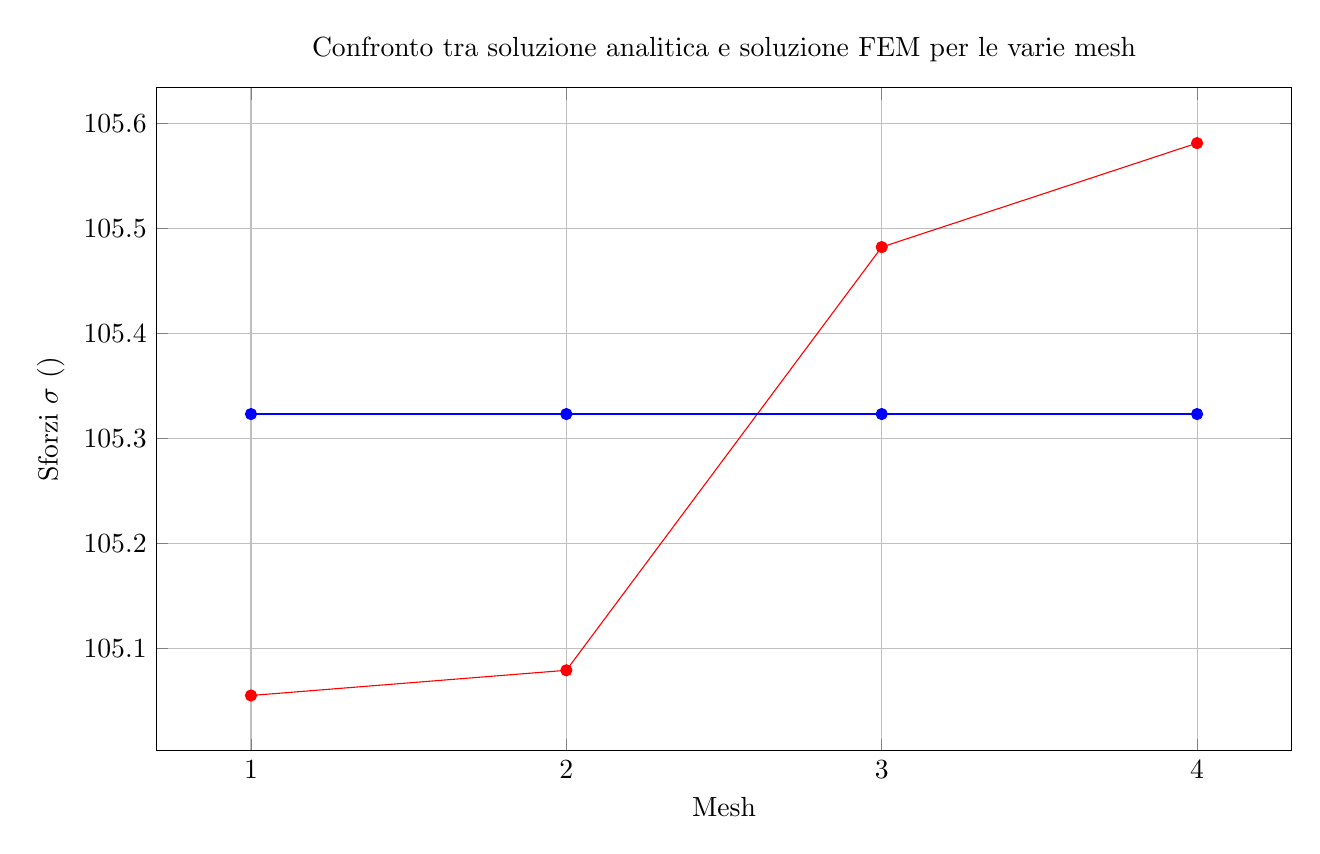
\begin{tikzpicture}\centering
	\begin{axis}[
	    height=10cm,
		width=16cm,
		grid=major,
		xlabel=Mesh,
		ylabel=Sforzi $\sigma$ (\si{\mega\pascal)},
		xtick = {1,2,3,4},
		title=Confronto tra soluzione analitica e soluzione FEM per le varie mesh
    ]
	\addplot[color=red,mark=*] coordinates {
		(1,105.055)
		(2,105.079)
		(3,105.482)
		(4,105.581)
	};
	\addplot[color=blue,mark=*] coordinates {
		(1,105.323)
		(2,105.323)
		(3,105.323)
		(4,105.323)
	};
	\end{axis}
\end{tikzpicture}
\end{center}